\documentclass[a4paper, 10pt]{article}
\usepackage{graphicx} % Required for inserting images
\usepackage[utf8]{inputenc}
\usepackage[german]{babel}
\usepackage{geometry}
\usepackage{fancyhdr}
\usepackage{titlesec}
\usepackage{xcolor}
\usepackage{enumitem}
\usepackage{lipsum}
\usepackage{tcolorbox}
\usepackage{amsmath} % Für mathematische Formeln (optional)
\usepackage{xcolor}  % Für Farbdefinitionen
\usepackage{soul}    % Für Textmarkierung

% Seitenlayout
\geometry{top=2.5cm, left=2cm, right=2cm}

% Kopf- und Fußzeile
\pagestyle{fancy}
\fancyhf{}
\fancyhead[L]{\textbf{Deutsches und internationales Unternehmensrecht 2024/25}}
\fancyhead[R]{\textbf{Lena Thuy Trang Vo}}
\fancyfoot[C]{\thepage}

% Farben (Mintgrün)
\definecolor{lightpastelmint}{rgb}{0.74, 0.96, 0.84}
\definecolor{darkpastelmint}{rgb}{0.47, 0.85, 0.62}

% Titel-Formatierung
\titleformat{\section}{\large\color{darkpastelmint}\bfseries}{}{0em}{}[\titlerule]
\titleformat{\subsection}{\color{darkpastelmint}\bfseries}{}{0em}{}

% Definition-Box
\newtcolorbox{Fall}{
  colback=lightpastelmint, % Hintergrundfarbe
  colframe=darkpastelmint, % Rahmenfarbe
  fonttitle=\bfseries,
  title=Fall,
  boxrule=0.8mm, % Dicke des Rahmens
  width=\textwidth, % Breite der Box
  before=\vspace{0.5cm}, % Abstand vor der Box
  after=\vspace{0.5cm}, % Abstand nach der Box
  sharp corners=south % Scharfe Ecken unten
}
\definecolor{highlightmint}{rgb}{0.74, 0.96, 0.84}
% Befehl für das Hervorheben
\sethlcolor{highlightmint} % Setze die Highlight-Farbe

\begin{document}

\begin{titlepage}
    \centering
    \vspace*{3cm}
    {\Huge \textbf{Deutsches und Internationales Unternehmensrecht}}\\[1.5cm]
    {\large \textit{Lena Thuy Trang Vo}}\\[0.5cm]
    {\large \textit{Wintersemester 2024/25}}\\[2cm]

    \vfill
\end{titlepage}

\tableofcontents
\newpage

\section{1. Einheit}
\subsection{Wovon handelt das Handelsrecht?}
\begin{itemize}
    \item das Handelsrecht ist ein \textbf{spezielles Teilgebiet} des Privatsrechts, da sich mit den \textbf{Rechtsbeziehungen zwischen Kaufleuten und Unternehmen} befasst
    \item  Handelsrecht regelt die Rechtsbeziehungen eines abgegrenzten Personenkreises, nämlich der Kaufleute
    \begin{itemize}
        \item \hl{Sonderprivatrecht der Kaufleute}
    \end{itemize}
    \item Handelsrecht \textbf{ergänzt} Bürgerliches Recht
    \item Handelsrecht \textbf{ändert} Bürgerliches Recht ab
\end{itemize}
\subsection{Bürgerliches Recht ergänzende Normen}
\textbf{\hl{Beispiel: gutgläubiger Eigentumserwerb}}
\begin{itemize}
    \item nach \hl{§ 932 BGB} kann jemand gutgläubig Eigentum an einer beweglichen Sache erwerben, wenn er beim Erwerb der Sache davon ausgeht, dass der Veräußerer der Eigentümer ist
    \item Handelsrecht ergänzt diese Regelung durch \hl{§ 366 HGB}, der speziell für den kaufmännischen Verkehr gilt
    \begin{itemize}
        \item bedeutet, dass ein gutgläubiger Erwerb auch dann möglich ist, wenn der Erwerber glaubt, dass der Veräußerer aufgrund einer Ermächtigung des Eigentümers zur Verfügung über die Sache befugt ist
    \end{itemize}
\end{itemize}
\subsection{Funktionen des Handeslrecht}
Funktionen sind darauf ausgerichtet, die \textbf{Effizienz und Sicherheit} im Geschäftsverkehr unter Kaufleuten zu fördern:
\begin{itemize}
    \item \hl{Schnelligkeit} und \hl{Einfachheit}
    \begin{itemize}
        \item Kaufleute schließen häufig eine \textbf{große Anzahl von Geschäften} ab, weshalb das Handelsrecht darauf abzielt, diese \textbf{Prozesse schnell und unkompliziert} zu gestalten
        \item Bsp. \hl{Mangelrügepflicht gemäß §377 HGB}, die eine zügige Prüfunf und Anzeige von Mängeln bei Warenlieferung erfordert, um den schnellen Geschäftsablauf nicht zu stören
    \end{itemize}

    \item \hl{Rechtssicherheit und Klarheit bei Rechtsgeschäften}
    \begin{itemize}
        \item Handelsrecht bietet durch das \textbf{Verkehrs- und Vertrauensschutzprinzip} sowie das \textbf{Rechtsscheinprinzip} eine erhöhte Rechtssicherheit
    \end{itemize}

    \item \hl{geringere Schutzbedürftigkeit}
    \begin{itemize}
        \item aufgrund ihrer Geschäftserfahrung benötigen Kaufleute \textbf{weniger Schutz als Verbraucher}
        \item weniger Einschränkungen der \textbf{Privatautonomie und mehr Selbstverantwortung}
    \end{itemize}
\end{itemize}

\subsection{Quellen des Handelsrecht}
\begin{itemize}
    \item \textbf{Unionsrecht:}
    \begin{itemize}
        \item das europäische Unionsrecht beeinflusst das deutsche Handelsrecht erheblich
        \item nationale Regelungen müssen im \hl{Einklang mit EU-Recht} stehen
        \item bei der Auslegung von Handelsgesetzen ist eine \hl{unionskonforme Interpretation} erforderlich
        \item betrifft insbesondere Bereiche wie den \textbf{Binnenmarkt} und den \textbf{freien Warenverkehr}
    \end{itemize}
   
    \item \textbf{Deutsches Recht:}
    \begin{itemize}
        \item die wichtigste nationale Rechtsquelle ist das HGB, insbesondere das \hl{erste und vierte Buch}, die sich mit dem \hl{Handelsstand} und den \hl{Handelsgeschäften} befasst
    \end{itemize}

    \item \textbf{Handelsgewohnheitsrecht:}
    \begin{itemize}
        \item \hl{ungeschriebene Regeln,} die sich aus langjähriger Praxis im Geschäftsverkehr entwickelt haben
        \item diese Gewohnheiten sind \hl{durch die Rechtssprechung anerkannt} und werden im Handel als \hl{verbindlich} betrachtet
    \end{itemize}


    \item \textbf{Handelsbräuche:}
    \begin{itemize}
        \item diese sind \hl{Verkehrssitten im Handel}, die bei der \hl{Auslegung von Willenserklärungen} berücksichtigt werden
        \item sind \hl{nicht gesetzlich kodifiziert}, aber als Auslegungshilfe anerkannt 
    \end{itemize}
\end{itemize}

\subsection{Aufbau des Handelsgesetzbuches}
\begin{figure}[h]
    \centering
    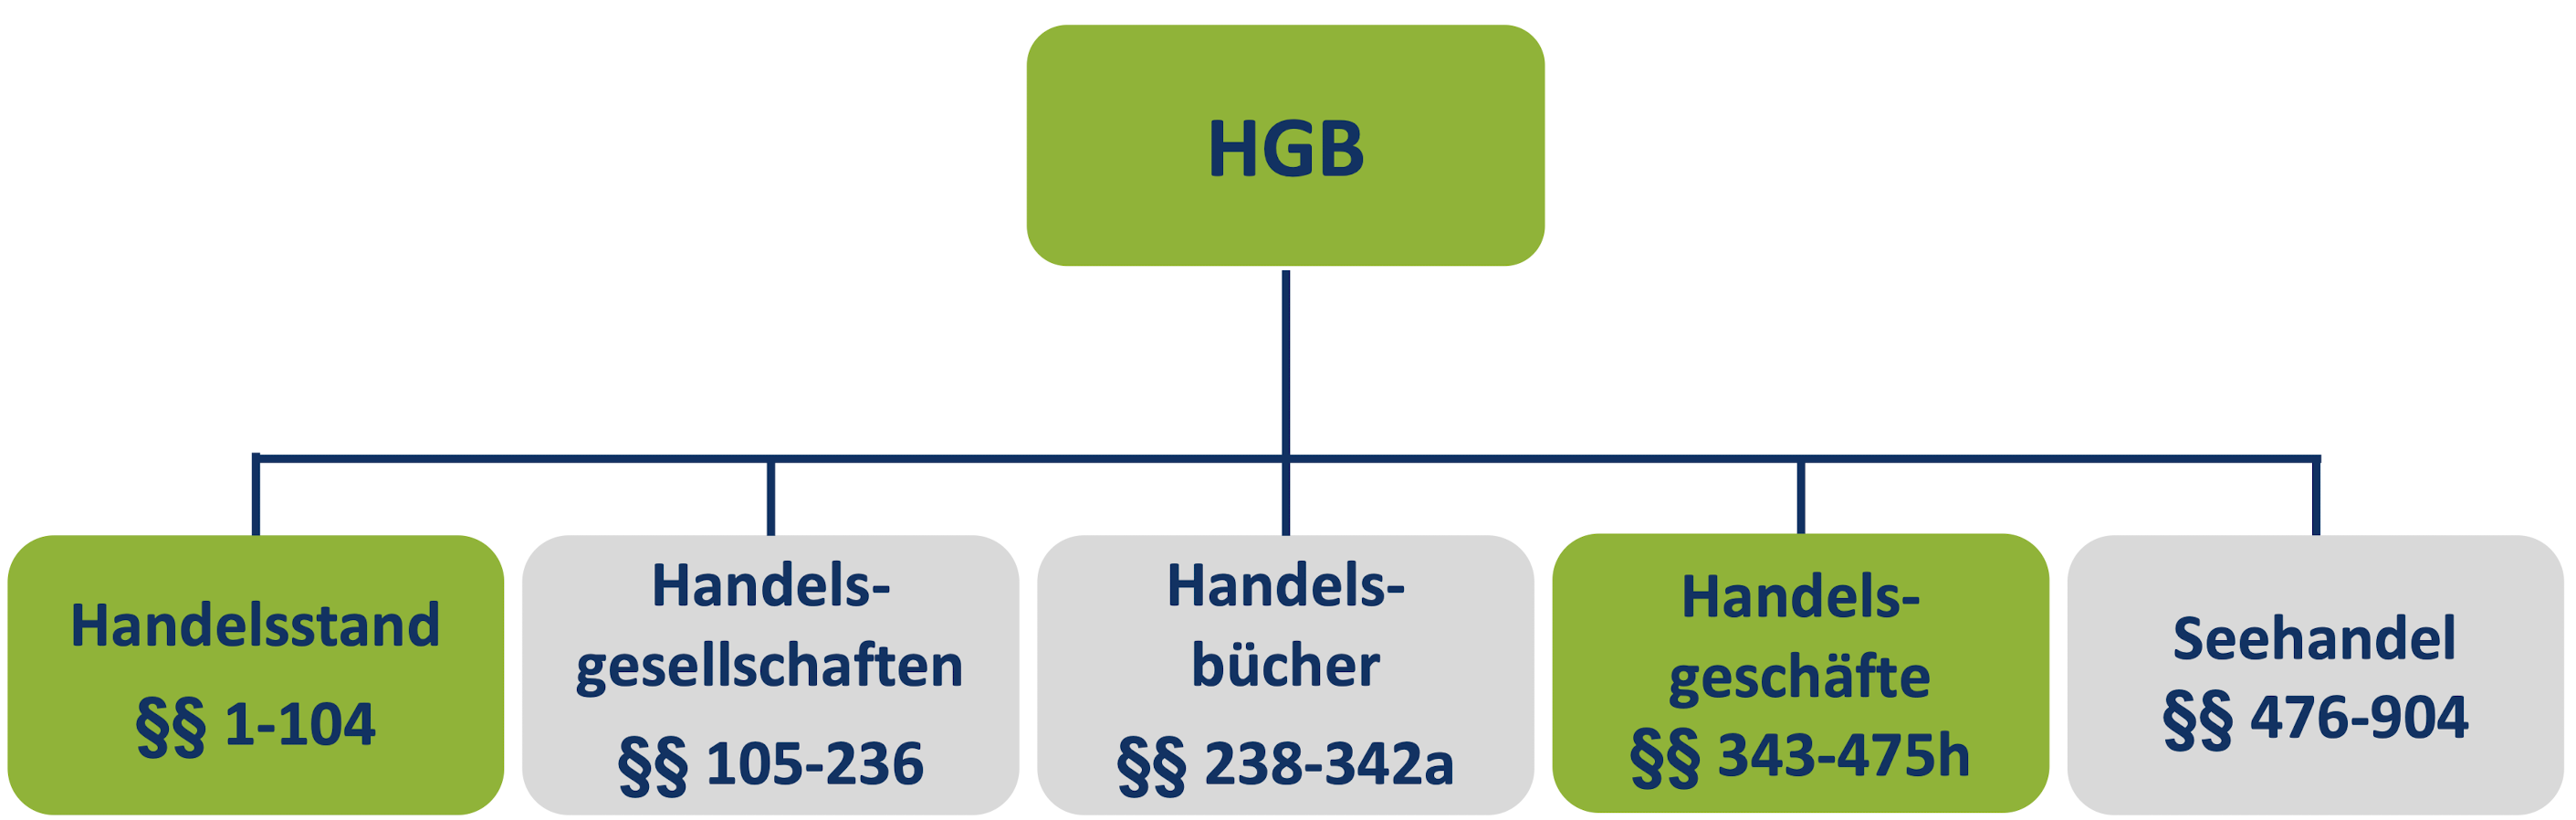
\includegraphics[width=0.6\linewidth]{Bildschirmfoto 2024-10-30 um 11.30.26.png}
    \caption{Aufbau HGB}
    \label{fig:enter-label}
\end{figure}

\subsection{Entstehungsgeschichte des Handelsrechts}
\begin{itemize}
    \item das \hl{ADHGB} wurde 1861 als erstes umfassendes Handelsgesetzbuch im deutschen Bund eingeführt
    \begin{itemize}
        \item es wurde als \textbf{Parallelgesetzgebung} in dne meisten deutschen Staaten erlassen und diente der \textbf{Vereinheitlichung} des Handelsrechts
    \end{itemize}
    \item war stark vom französischen \textbf{Code de Commerce} von 1807 beeinflusst
    \item nach der Gründung des Deutschen Reichs 1871 wurde das ADHGB als \textbf{Reichsgesetz} übernommen
    \begin{itemize}
        \item das stellte die erste gesamtdeutsche Kodifikation des Handelsrecht dar
    \end{itemize}

    \item die einheitliche Handhabung wurde durch das \textbf{Reichsoberhandelsgericht (ROHG} ab 1869 und später durch das \textbf{Reichsgericht} ab 1879 gewährleistet

    \item am \textbf{1. Januar 1900} trat das HGB gemeinsam mit dem BGB in Kraft

    \item 1937 wurde das \textbf{Aktienrecht kodifiziert}
    \item \textbf{große Novelle von 1965}
    \item \textbf{Handelsrechtkonformgesetz von 1998}
    \begin{itemize}
        \item Firmenrecht und Definition des Kaufmannsbegriffs
    \end{itemize}
\end{itemize}

\subsection{Der Kaufmannsbegriff}
Entscheidend für die \textbf{Anwendbarkeit des HGB} und damit für die \textbf{rechtlichen Rahmenbedinungen}, unter denen Geschäftsaktivitäten stattfinden
\begin{itemize}
    \item \textbf{statusbegründeter Anknüpfungspunkt}
    \begin{itemize}
        \item richtet sich primär an Kaufleute
        \item nur wer als Kaufmann gilt, unterliegt den besonderen Vorschriften des HGB
    \end{itemize}

    \item die Kaufmannseigenschaft \textbf{mindestens eines der Beteiligten} ist erforderlich, damit das HGB auf ein Rechtsgeschäft oder eine Rechtsbeziehung Anwendung findet

    \item nach \hl{§1 HGB} ist ein Kaufmann, wer ein \textbf{Handelsgewerbe} betreibt
    \begin{itemize}
        \item ein Handelsgewerbe ist \textbf{jedes Gewerbe}, das nach Art und Umfang einen in \textbf{kaufmännischer Weise} eingerichteten Geschäftsbetrieb erfordert
    \end{itemize}

    \item nicht jeder Gewerbetreibende ist ein Kaufmann 
    \begin{itemize}
        \item entscheidend ist, ob das Gewerbe so groß und komplex ist, dass es eine \textbf{professionelle Betriebsführung} erfordert
        \item kleinere Gewerbebetriebe, die keinen kaufmännisch eingerichteten Geschäftsbetrieb benötigen, gelten nicht als Handelsgewerbe und somit nicht als Kaufleute im Sinne des HGB
    \end{itemize}

    \item \hl{Kannkaufmann § 2, 3 Abs. 2
HGB}
    \begin{itemize}
        \item ist ein Gewerbetreibender, der sich \textbf{freiwillig ins Handelsregister} eintragen lässt, obwohl er \textbf{nicht dazu verpflichtet} ist
        \item diese Eintragung verleiht im die Kaufmannseigenschaft mit allen Rechten und Pflichten des HGB
    \end{itemize}
\end{itemize}
\subsection{Schematische Darstellung des Kaufmannsbegriffs}
\begin{figure}[h]
    \centering
    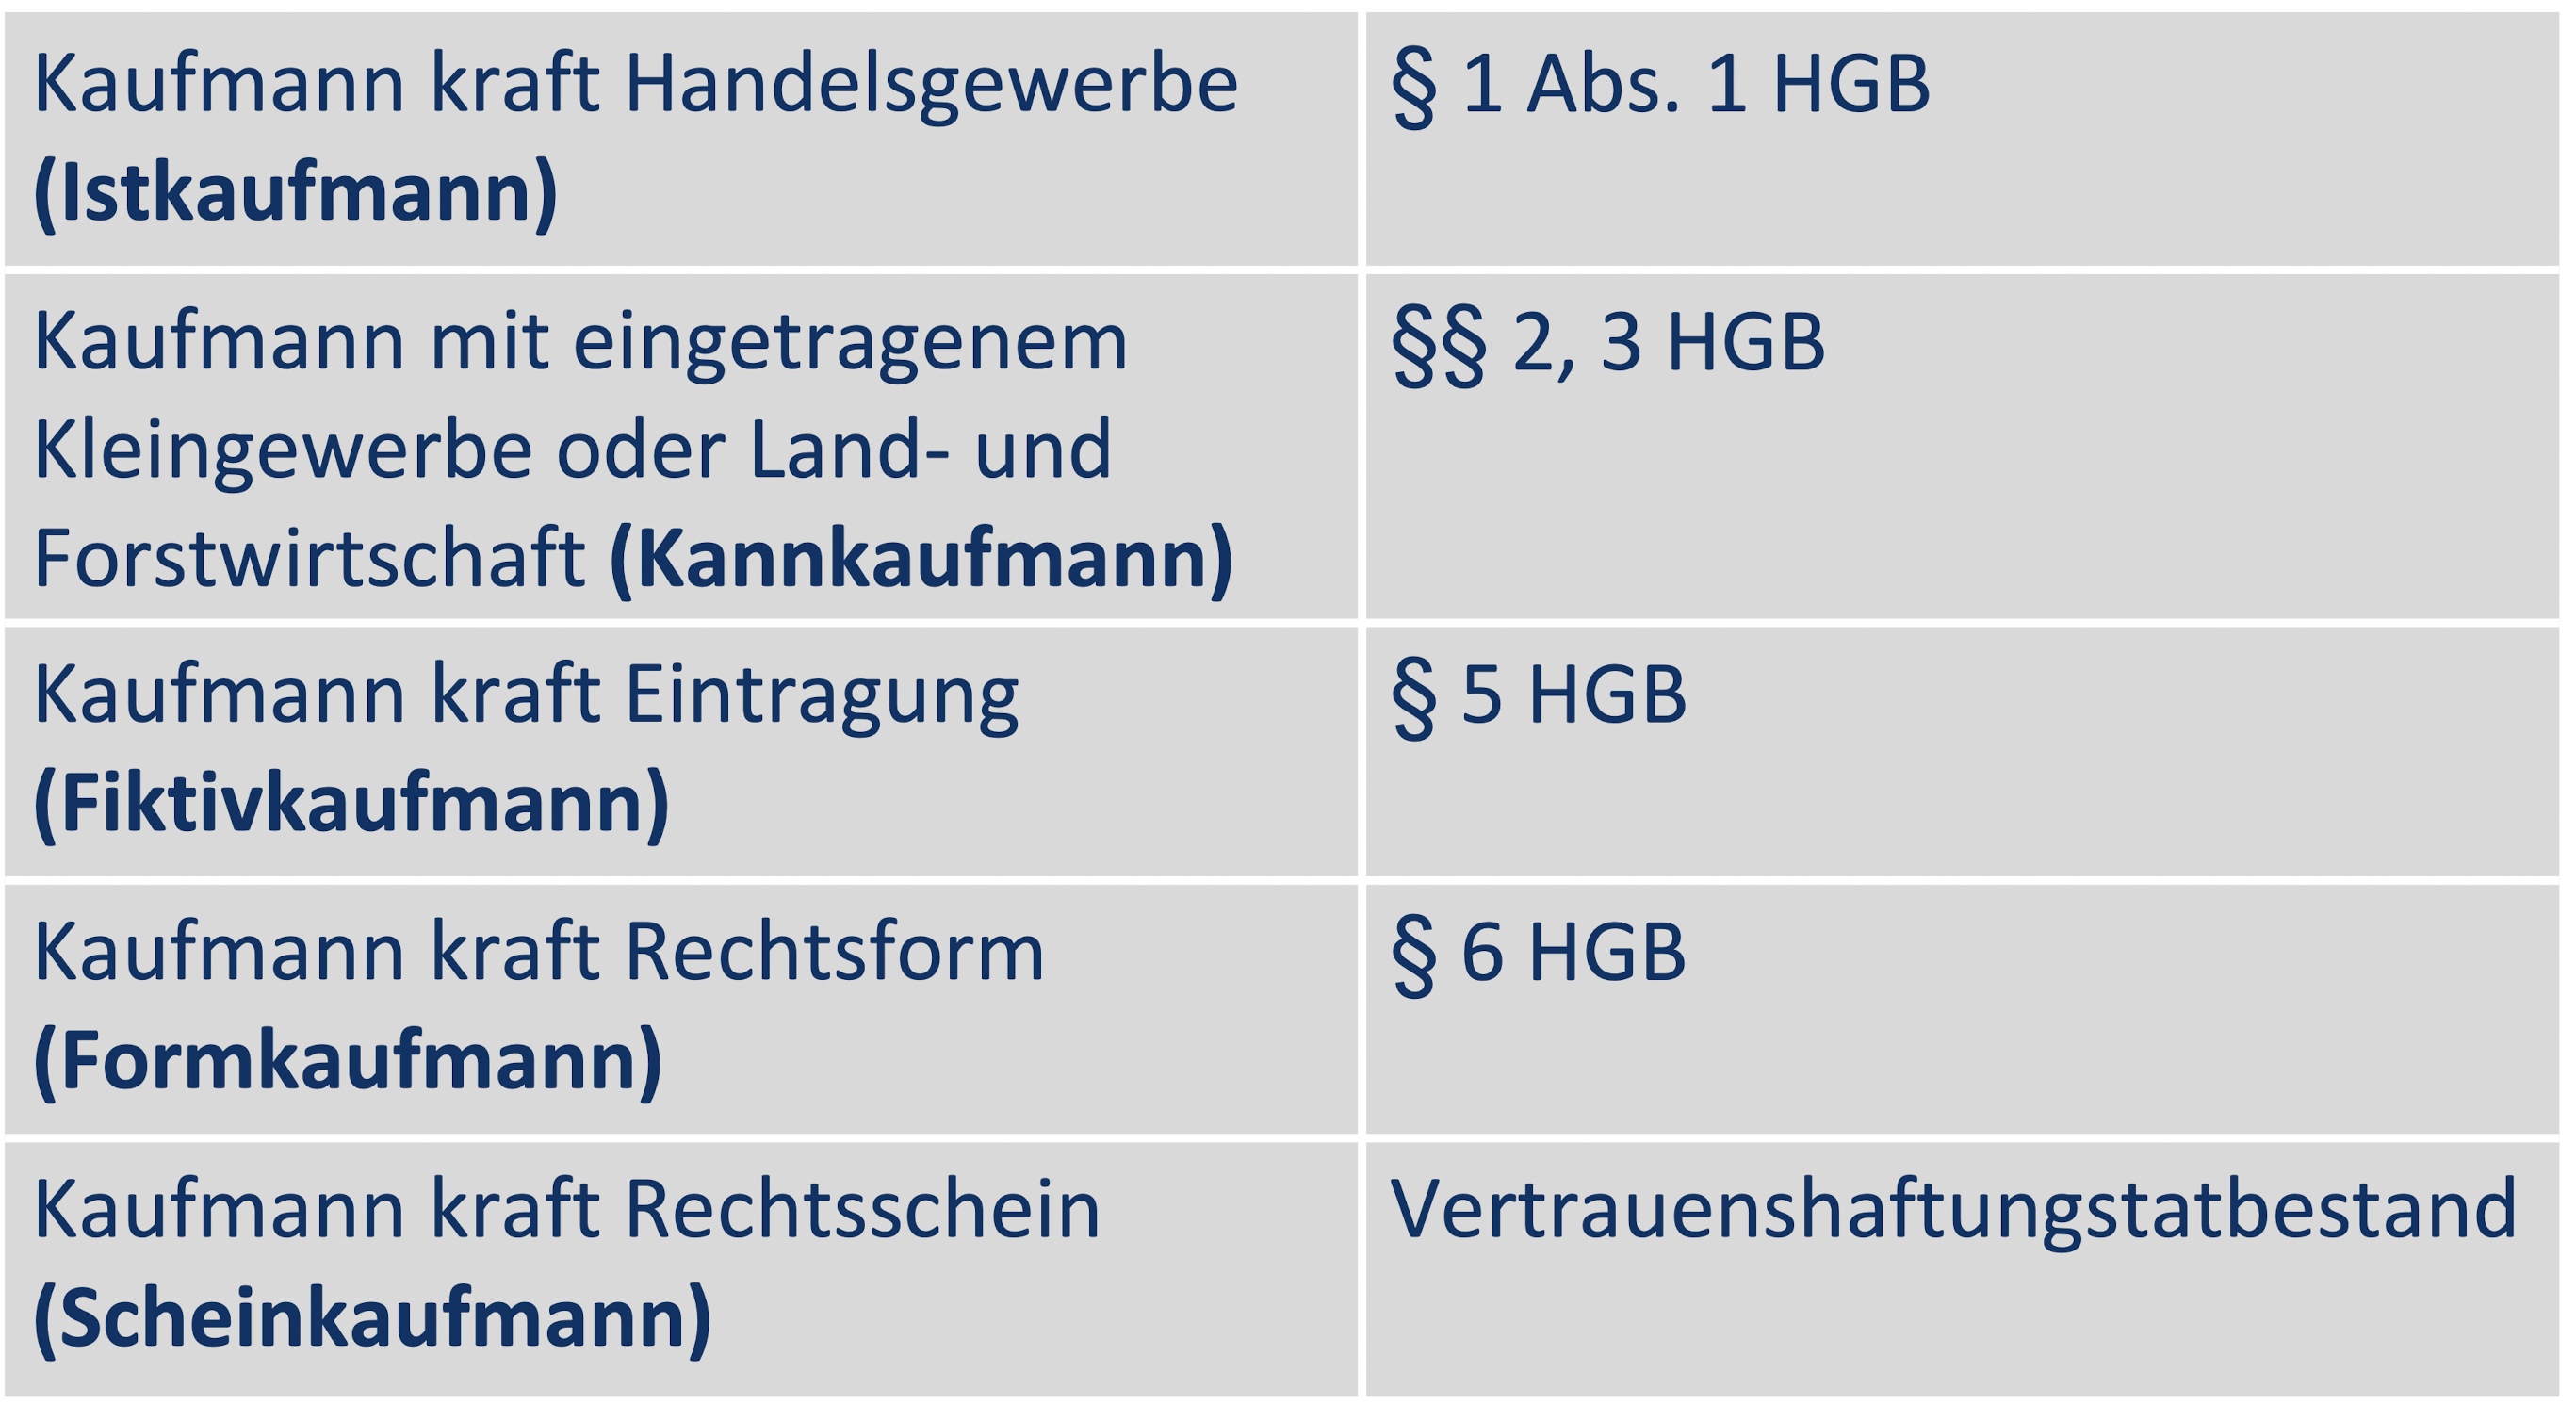
\includegraphics[width=0.5\linewidth]{Bildschirmfoto 2024-10-30 um 12.09.16.png}
    \caption{Kaufmannsbegriff}
    \label{fig:enter-label}
\end{figure}
\subsection{Widerholungsfragen für die nächste Einheit}
\begin{enumerate}
    \item Wie verhalten sich HGB und BGB zueinander\\[2.5mm]
    Das HGB \textbf{ergänzt oder ändert} das BGB ab. Das HGB enthält spezielle Regelungen, die \textbf{Vorrang} vor den allgemeinen Bestimmtungen des BGB haben. Wo das HGB hingegen keine speziellen Vorschriften enthält, wird auf die \textbf{allgemeinen Regelungen des BGB zurückgegriffen}.

    \item Was folgt daraus für die Falllösung (Verknüpfung mit dem
allgemeinen Zivilrecht)?
\begin{enumerate}
    \item Vorrangige Prüfunf der Spezialvorschriften des HGB (insb. Kaufmannseigenschaft)
    \item \textbf{Subsidäre Anwendung} der allgemeinen Prinzipien des BGB, wenn das HGB keine speziellen Regelungen enthält.
\end{enumerate}

\end{enumerate}
\section{2. Einheit}
\subsection{Ist-Kaufmann}
\begin{itemize}
    \item bescheibt eine Person, die kraft Gesetzes Kaufmann ist, weil sie ein \hl{Handelsgewerbe} betreibt
    \item um als IstKaufmann gemäß \hl{§ 1 Abs. 1 HGB} zu gelten, müssen zwei wesentliche Kriterien erfüllt sein
    \begin{enumerate}
        \item es muss ein \textbf{Gewerbe} vorliegen
        \item \textbf{Handelsgewerbe}
        \begin{enumerate}
            \item achtung, nicht jedes Gewerbe ist ein Handelsgewerbe
            \item gemäß \hl{§ 1 Abs. 2 HGB} wird ein Gewerbe zum Handelsgewerbe, wenn es nach Art und Umfang einen \textbf{in kaufmännischer Weise eingerichteten Geschäftsbetrieb} erfordert
        \end{enumerate}
    \end{enumerate}

    \begin{figure}[h]
        \centering
        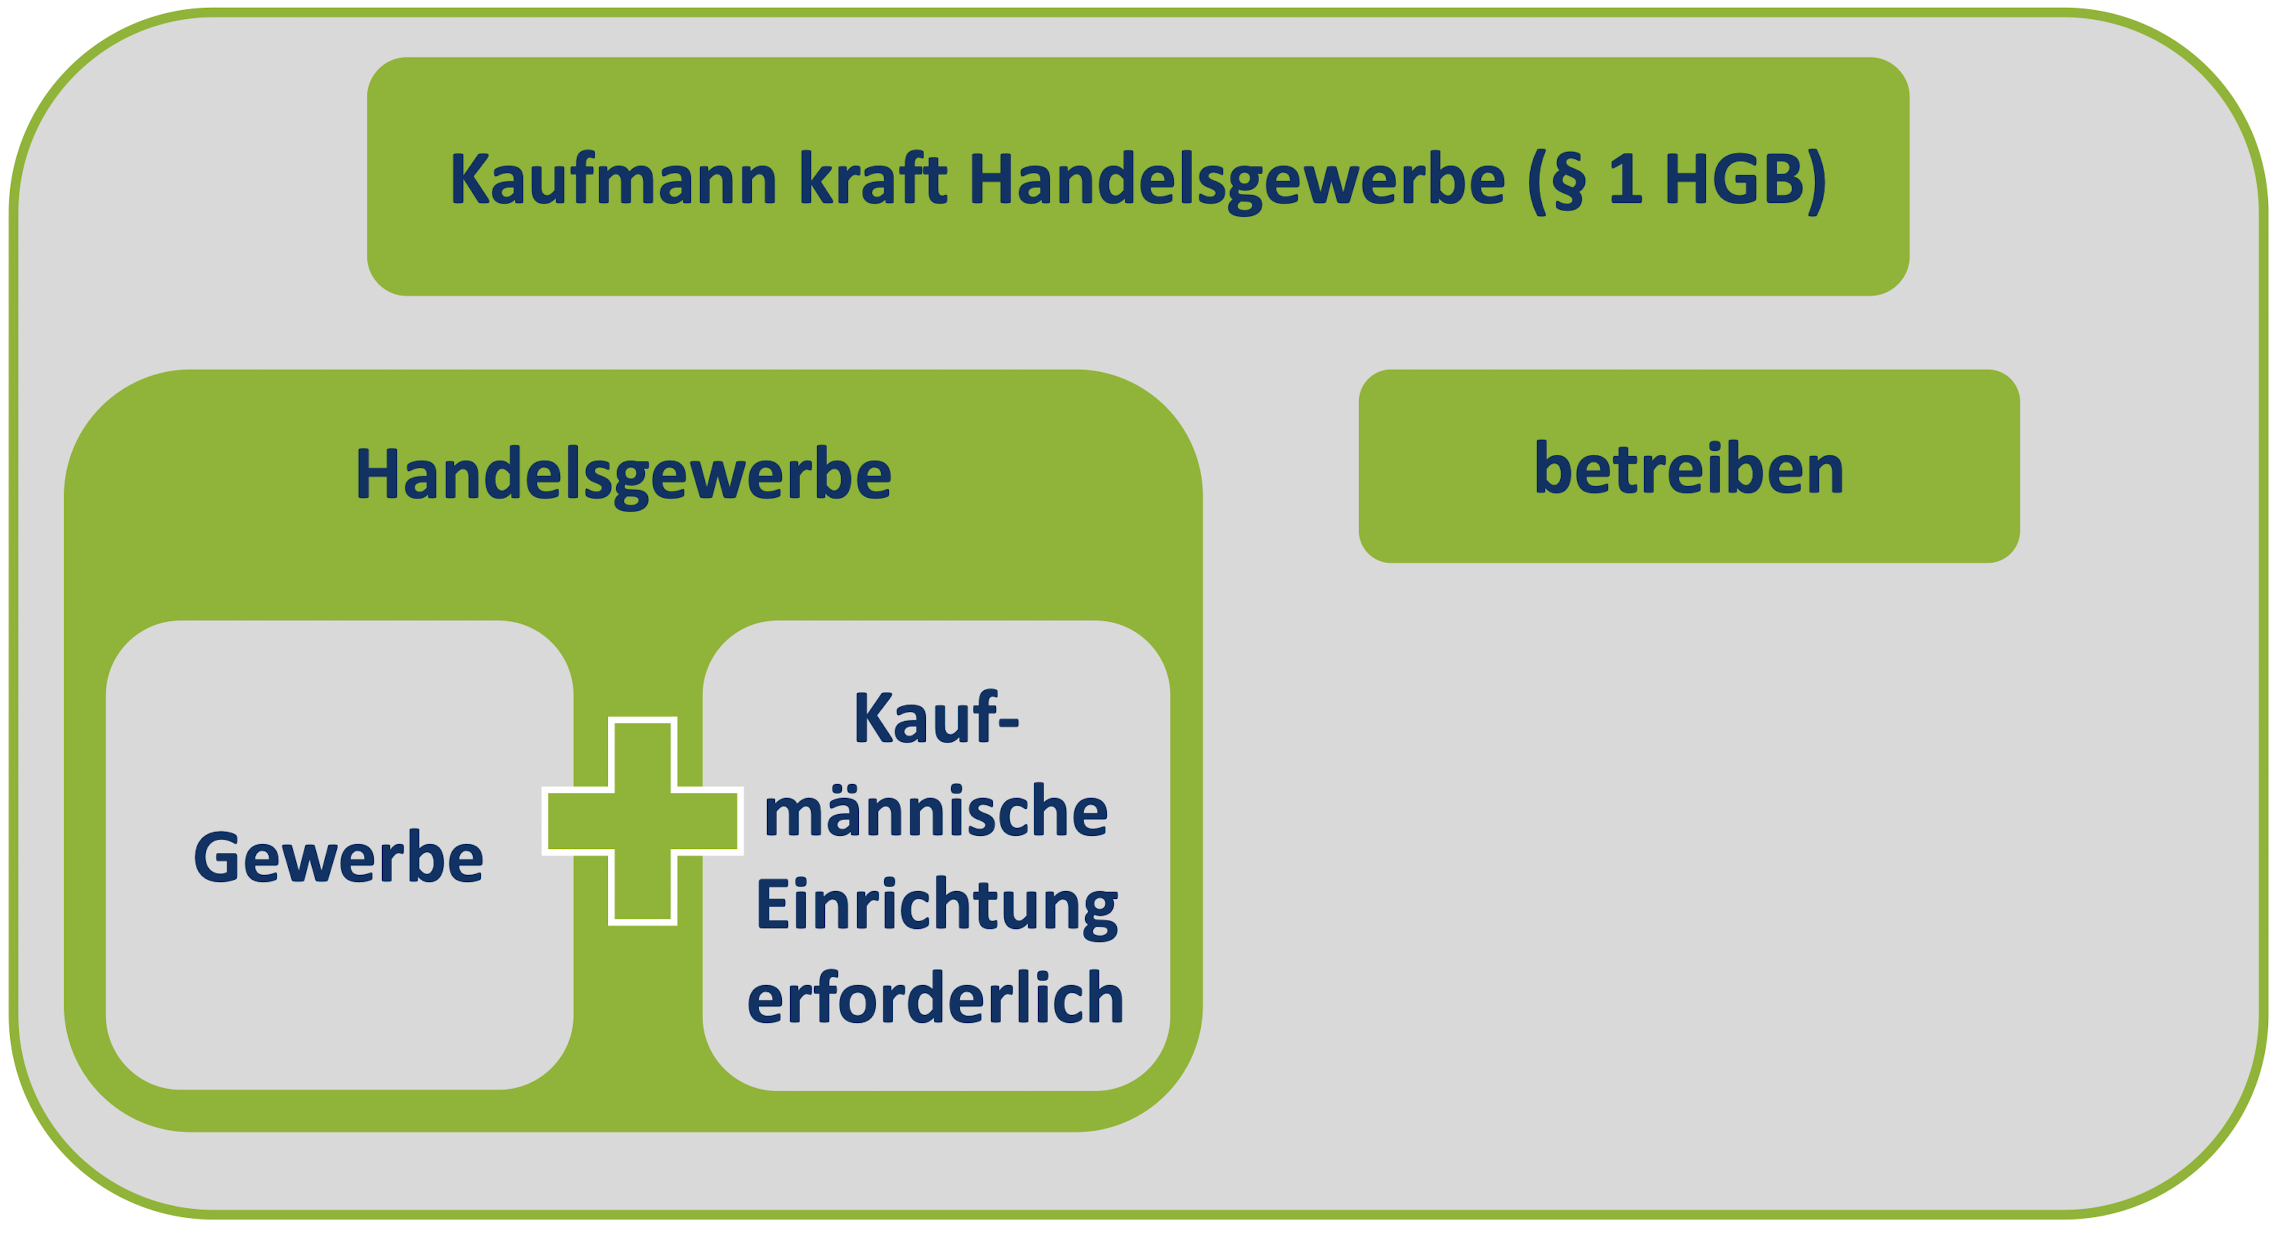
\includegraphics[width=0.5\linewidth]{Bildschirmfoto 2024-10-30 um 12.28.37.png}
        \caption{IstKaufmann}
        \label{fig:enter-label}
    \end{figure}
\end{itemize}
\subsection{Gewerbe}
ist eine Tätigkeit, die
\begin{itemize}
    \item \textbf{rechtlich selbstständig},
    \item \textbf{entgeltlich} bzw. mit Gewinnerzielungsabsicht
    \item \textbf{planmäßig} und \textbf{dauerhaft} (=Vielzahl von Geschäften),
    \item auf \textbf{wirtschaftlichem Gebiet = nicht freiberuflich} (nicht wissenschaftlich, lehrend, künstlerisch, sportlich, gemeinnützig) und
    \item \textbf{am Markt} (äußerlich erkennbar) ausgeübt wird.
\end{itemize}
\hl{\textbf{nicht erfasste Tätigkeiten}}
\begin{itemize}
    \item \textbf{unselbstständige Tätigkeiten:}
    \begin{itemize}
        \item Arbeitnehmer sind \textbf{nicht selbstständig tätig}, auch wenn sie in leitenden Positionen arbeiten
        \item handeln im Auftrag und unter der \textbf{Weisung eines Arbeitgebers} und tragen \textbf{nicht das wirtschaftliche Risiko} 
        \item \hl{§ 84 Abs. 1 Satz 2 HGB}
    \end{itemize}

    \item \textbf{Freiberufliche Tätigkeiten:}
    \begin{itemize}
        \item zeichnen sich durch die \textbf{Erbringung höchstpersönlicher Leistungen}aus, die in der Regel eine \textbf{besondere Qualifikation} oder \textbf{schöpferische Tätigkeit} erfordern

        \item Ein Anhaltspunkt für die \textbf{Zuordnung zu den freien Berufen} findet sich in \hl{§ 1 Abs. 2 }des \textbf{Partnerschaftsgesellschaftsgesetzes (PartGG)}, das typische freie Berufe auflistet.
    \end{itemize}
\end{itemize}

\noindent\textbf{\hl{Gewerbe != freiberufliche Tätigkeit}}
\begin{itemize}
    \item entscheidend ist die \textbf{freiberufliche Prägung} der Tätigkeit
\end{itemize}
\newpage
Beispiele: 
\begin{itemize}
    \item Ein Arzt, der ein Sanatorium betreibt, verlagert den Schwerpunkt von der ärztlichen Tätigkeit auf den Betrieb einer größeren Einrichtung.
    \item Ein Architekt, der ein technisches Büro führt, entfernt sich von der rein entwerfenden Tätigkeit.
    \item Ein Künstler, der in großem Umfang Kunstwerke für den Markt produziert, bewegt sich weg von individuellen Schöpfungen hin zu gewerblichen Produktionen.
\end{itemize}
\begin{Fall}
    Die Prima-Kost GmbH beschäftigt als Außendienstverkäufer
unter anderem Andreas.\\
In seinem Vertrag mit der GmbH wird er als \textbf{selbständiger
Gewerbetreibender} bezeichnet.\\
Tägliche Fahrtroute, Kundenliste, Verkaufspreise und alle
Details werden ihm \textbf{von der GmbH genau vorgeschrieben}.\\
Eigenen \textbf{unternehmerischen Spielraum hat er nicht}.
\end{Fall}
Ist Andreas Kaufmann kraft Handelsgewerbe?\\[2mm]
Nein, da er \textbf{nicht rechtlich selbstständig} ist. Er handelt im Auftrag und unter Weisung eines Arbeitgebers und trägt somit nicht das wirtschaftliche Risiko.\\[2mm]

\noindent\begin{Fall}
    Barbara hat hinter ihrem Haus einen großen Obstgarten.
\textbf{Zur Zeit der Apfelernte} setzt sie sich mit einem Verkaufsstand
an die Straße.
\end{Fall}
Ist Barbara Kauffrau?\\[2mm]
Nein, weil es \textbf{nicht dauerhaft} ist, sondern nur zur Erntezeit, also \textbf{saisonal}.

\subsection{Unternehmer}
\begin{itemize}
    \item \hl{Wer Kaufmann ist, ist auch Unternehmer}
    \item Begriff des Unternehmers gemäß \hl{§ 14 BGB} ist weiter gefasst als der des Kaufmanns im Sinne des HGB
    \item \hl{nicht jeder Unternehmer ist zugleich Kaufmann!}
    \begin{itemize}
        \item da der Unternehmerbegriff auch Tätigkeiten umfasst, die nicht die Kriterien eines Handelsgewerbes erfüllen.
    \end{itemize}

    \item Unternehmerbegriff ist \textbf{autonom} und orientiert sich an den \textbf{Vorgaben des europäischen Rechts}
    \item est nicht an den traditionellen deutschen Gewerbebegriff gebunden, was zu einer breiteren Anwendung führt
\end{itemize}

\begin{figure}[h]
    \centering
    
\includegraphics[width=0.5\linewidth]{Bildschirmfoto 2024-10-30 um 13.10.17.png}
    
    \label{fig:enter-label}
\end{figure}
\subsection{Unternehmen und Unternehmer}
\textbf{\hl{Unternehmer}}
\begin{itemize}
    \item ist eine Person, die ein \textbf{Unternehmen betreibt}
    \item dies kann eine \textbf{natürliche Person} (z.B. ein Einzelunternehmer) oder eine \textbf{juristische Person} (z.B. eine GmbH oder AG) sein
    \item Unternehmer ist das \textbf{Rechtssubjekt}, das die \textbf{rechtlichen Handlungen} im Namen des Unternehmens vornimmt und für dessen \textbf{Verpflichtungen haftet}
\end{itemize}

\noindent\textbf{\hl{Unternehmen}}
\begin{itemize}
    \item ein Unternehmen umfasst alle \textbf{materiellen und immateriellen} Vermögenswerte, die dem \textbf{Unternehmenszweck} gewidmet sind (Sondervermörgen)
    \item ist eine \textbf{organisatorische und wirtschaftliche Einheit}, die durch einen bestimmten \textbf{Zweck} definiert ist 
    \item ein Unternehmen selbst ist \textbf{kein Rechtssubjekt}, d.h. es kann nicht Träger von Rechten und Pflichten sein
\end{itemize}

\subsection{Kannkaufmann}
\textbf{\hl{Kleingewerbetreibender}}
\begin{itemize}
    \item betreiben ein \textbf{Gewerbe}, das unterhalb der \textbf{Mindestgrößanforderungen} für einen in kaufmännischer Weise eingerichteten Geschäftsbetrieb liegt
    \item da der Betrieb diese Anforderungen nicht erfüllt, ist ein \textbf{kaufmännisch eingerichteter Geschäftsbetrieb} nicht erforderlich
    \item haben die Möglichkeit, durch \textbf{freiwillige Eintragung ins Handelsregister} die Kaufmannseigenschaft zu erlangen
    \item Kaufmannseigenschaft wird durch den \textbf{Staatsakt der Eintragung} ins Handelsregister erworben 
    \item bei der Eintragung wird die \textbf{Betriebsgröße nicht geprüft}
\end{itemize}

\textbf{Unterschiede in der Eintragung:}
\begin{enumerate}
    \item \hl{zwingende, deklarative Eintragung (§§ 1 Abs.2, 29 HGB)}
    \begin{itemize}
        \item Betriebe, die einen in kaufmännischer Weise eingerichteten Geschäftsbetrieb erfordern, sind verpflichtet, sich ins Handelsregister eintragen zu lassen
    \end{itemize}

    \item \hl{Freiwillige Eintragung (§2 HGB)}
    \begin{itemize}
        \item Kleingewerbetreibende, deren Betriebe keinen kaufmännisch eingerichteten Geschäftsbetrieb erfordern, können sich freiwillig ins Handelsregister eintragen lassen
    \end{itemize}
\end{enumerate}

\noindent\textbf{\hl{kaufmännisch eingerichteter Geschäftsbetrieb}}
\begin{itemize}
    \item umfasst alle organisatorischen und technischen Einrichtungen, die \textbf{erforderlich} sind, um eine ordentliche, übersichtliche und zuverlässige \textbf{Geschäftsführung zu gewährleisten}
\end{itemize}
\textbf{Kritierien zur Bewertung:}
\begin{enumerate}
    \item \hl{Art des Gewerbebetriebs}

    \begin{itemize}
        \item Natur und Vielfalt der Geschäfte, welche Erzeugnisse oder Dienstleistungen angeboten werden und wie vielfältig diese sind
    \end{itemize}

    \item \hl{Umfang des Gewerbebetriebs (Betriebsgröße)}
    \begin{itemize}
        \item Anlage- und
Betriebskapital, Umsatz, Kreditbedarf, Zahl der
Beschäftigten, Betriebsstätten, Lagerhaltung etc.
    \end{itemize}
\end{enumerate}

\textbf{\hl{Löschung eines Kannkaufmanns}}
\begin{itemize}
    \item unter \textbf{bestimmten Bedingungen} möglich und bietet eine Art \textbf{„Rückfahrkarte“} für Kleingewerbetreibende
    \item kann gemäß \hl{§ 2 Satz 3 HGB} beantragen, im Handelsregister gelöscht zu werden
    \item ist nur möglich, wenn der Betrieb \textbf{nicht die Größengrenze überschritten} hat, die ihn zum \textbf{Ist-Kaufmann} machen würde
    \item wenn die \textbf{"Gewerblichkeit"} eines Unternehmens vollständig wegfällt, kann eine \textbf{amtswegige Löschung} erfolgen

    \item wenn ein Istkaufmann unter die Größengrenze fällt, wird er wieder zum Kannkaufmann
    \begin{itemize}
        \item keine automatische Löschung aus dem Handelsregister
        \item hat Option, als Kannkaufmann im Handelsregister zu bleiben oder die Löschung zu bentragen
    \end{itemize}
\end{itemize}

\textbf{\hl{Land- und Forstwirt}}
\begin{itemize}
    \item Land- und Forstwirte sind \textbf{niemals Ist-Kaufleute} im Sinne des \hl{§ 1 HGB}
    \item Wird die Land- oder Forstwirtschaft jedoch in der Rechtsform einer \textbf{Kapitalgesellschaft oder Genossenschaft} betrieben (z.B. GmbH, AG), gelten sie als \textbf{Formkaufmann} gemäß \hl{§ 6 Abs. 2 HGB}, unabhängig von der Art des Betriebs
    \item können sich \textbf{freiwillig} ins Handelsregister eintragen lassen und dadurch die Kaufmannseigenschaft erwerben \hl{§ 3 Abs. 2 HGB}
    \item Entscheiden sich Land- und Forstwirte \textbf{gegen die Eintragung}, unterliegen sie nicht den Vorschriften des HGB, sondern dem \textbf{allgemeinen Bürgerlichen Recht (BGB)}
\end{itemize}

\subsection{Fiktivkaufmann}
\begin{itemize}
    \item \textbf{Kaufmann kraft Eintragung} gemäß \hl{§ 5 HGB}
    \item beschreibt eine Situation, in der eine im Handelsregister eingetragene Firma \textbf{als Kaufmann behandelt} wird, selbst wenn das zugrunde liegende Gewerbe \textbf{nicht die Merkmale eines Handelsgewerbes} erfüllt
    \item \hl{§ 5 HGB} fingiert die Kaufmannseigenschaft für denjenigen, dessen \textbf{Firma im Handelsregister} eingetragen ist
    \item bedeutet, dass unabhängig davon, ob das Gewerbe tatsächlich ein Handelsgewerbe im Sinne des \hl{§ 1 Abs. 2 HGB} ist, der \textbf{Eingetragene als Kaufmann} behandelt wird
    \item Regelung dient der \textbf{objektiven Rechtssicherheit} und dem \textbf{absoluten Verkehrsschutz}
    \item Fiktion der Kaufmannseigenschaft greift unabhängig davon, ob der Einegtragene die Eintragung \textbf{selbst veranlasst} hat oder überhaupt \textbf{von ihr weiß}
    \item \hl{§ 5 HGB} ist \textbf{keine Rechtsscheinnorm}
    \begin{itemize}
        \item bedeutet, dass die Fiktion der Kaufmannseigenschaft \textbf{nicht auf dem Vertrauen Dritter} basiert 
        \item selbst wenn ein \textbf{Vertragspartner} weiß, dass \textbf{kein Handelsgewerbe vorliegt}, bleibt die Fiktion bestehen 
    \end{itemize}
    \item keine Ausprägung des Scheinkaufmanns
    \item für die Anwendung des § 5 HGB muss zumindest ein Gewerbe vorliegen
    \begin{itemize}
        \item die Vorschrift fingiert nur das Vorliegen eines Handelsgewrbesm nicht jedoch eines Gewerbes an sich
        \item daher wird ein versehentlich eingetragener Freiberufler nicht erfasst, da Freiberufler per Definition kein Gewerbe betreiben
    \end{itemize}
\end{itemize}
\subsection{Formkaufmann}
gemäß \hl{§ 6 HGB}\\[2.5mm]
\textbf{\hl{Handelsgesellschaften}}
\begin{itemize}
    \item Handelsgesellschaften unterliegen gemäß \hl{§ 6 Abs. 1 HGB} den
\textbf{Regeln für Kaufleute}
\item innerhalb der Handelsgesellschaften sind zwei Gruppen zu unterscheiden:
\begin{itemize}
    \item \textbf{Personenhandelsgesellschaften}, deren Kaufmannseigenschaft
sich aus dem Betrieb eines \hl{Handelsgewerbes} ergibt
\item \textbf{Handelsgesellschaften} kraft Rechtsform, bei denen die
Kaufmannseigenschaft auf einer \hl{gesetzlichen Anordnung}
beruht (Kapitalgesellschaften = Formkaufleute)
\end{itemize}

\item Kapitalgesellschaften haben gegenüber Personengesellschaften den Vorteil, dass die Gesellschafter \textbf{nicht persönlich für die Verbindlichkeiten der Gesellschaft haften}

\item Kapitalgesellschaften entstehen nicht bereits mit dem
Vertragsschluss der Gesellschafter, sondern erst mit der \textbf{Eintragung ins Handelsregister}
\begin{itemize}
    \item mit der Eintragung erlangen sie \textbf{Rechtsfähigkeit} als juristische Personen
\end{itemize}
\item Personengesellschaften besitzen eine \textbf{Teilrechtsfähigkeit}

\item gemäß \hl{§ 13 Abs. 3 GmbHG und § 3 Abs.1 AktG} sind GmbHs und AGs unabhängig von ihrem Geschäftszweck oder der Art ihrer Tätigkeit als \hl{Handelsgesellschaften} eingestuft
\begin{itemize}
    \item \textbf{Kaufleute kraft Rechtsform}
\end{itemize}
\item Für GmbHs und AGs \textbf{spielt es keine Rolle}, ob sie tatsächlich ein Handelsgewerbe betreiben
\begin{itemize}
    \item \textbf{gesetzliche Regelung} ordnet zwingend an, dass sie \textbf{als Handelsgesellschaften zu gelten haben}, was ihnen die Kaufmannseigenschaft verleiht
\end{itemize}
\item \hl{§ 6 Abs. 2 HGB} stellt klar, dass diese Regelung \textbf{nicht nur für Vereine} gilt, sondern für alle Körperschaften, die als juristische Personen organisiert sind.
\end{itemize}

\subsection{Scheinkaufmann}
\begin{itemize}
    \item \textbf{allgemeinen Rechtsscheingrundsätze} besagen, dass jemand, der \textbf{zurechenbar einen Rechtsschein geschaffen} hat, sich gegenüber gutgläubigen Dritten an diesem festhalten lassen muss
    \item Lehre vom Scheinkaufmann greift nur \textbf{subsidiär} zu allen anderen
Kaufmanns-Tatbeständen
\item ist eine Person ins \textbf{Handelsregister eingetragen}, geht der
\textbf{Fiktivkaufmann} gemäß \hl{§ 5 HGB} dem Scheinkaufmann vor
\item Tatbestand des Scheinkaufmanns kommt nur dann zur Anwendung, wenn \textbf{andere Kaufmannstatbestände nicht greifen}, insbesondere wenn die eingetragene Person \textbf{überhaupt nicht gewerblich tätig} ist.
\begin{itemize}
    \item Beispiel:\textbf{eingetragener Freiberufler}, da \hl{§ 5 HGB} lediglich das Vorliegen eines Handelsgewerbes fingiert,\textbf{ nicht jedoch das Vorliegen eines Gewerbes} an sich
\end{itemize}
\end{itemize}

\noindent\textbf{\hl{Rechtsscheintatbestand}} = Auftreten als Kaufmann, z.B durch
\begin{itemize}
    \item \textbf{ausdrückliche Erklärung}
    \begin{itemize}
        \item kann sowohl mündlich, als auch schriftlich erfolgen, schafft einen \textbf{klaren Rechtsschein}
    \end{itemize}

    \item \textbf{Verwendung kaufmännischer Einrichtungen}
    \begin{itemize}
        \item z.B durch Erteilung einer Prokura (kann nur von Kaufleuten erteilt werden)
    \end{itemize}
    \item Personen, die \textbf{kein Gewerbe} betreiben (z.B. Freiberufler), müssen einen \textbf{\hl{doppelten Rechtsschein}} setzen, um als Scheinkaufmann zu gelten
    \begin{itemize}
        \item sowohl den \textbf{Anschein eines Gewerbebetriebs} als auch den \textbf{Anschein einer Mindestbetriebsgröße} erwecken, die einen kaufmännsich eingerichteten Geschäftsbetrieb erfordert
    \end{itemize}
\end{itemize}
\textbf{Veranlassung des Rechtsscheintatbestandes:}
\begin{itemize}
    \item kann durch das \hl{eigene Verhalten} einer Person erzeugt werden (unerheblich, ob ein Verschulden vorliegt)
    \item kann auch entstehen, wenn eine Personn einen von \hl{Dritten erzeugten Anschein} kennt und duldet
    \begin{itemize}
        \item bedeutet, dass die Person den Anschein bewusst bestehen lässt, ohne dagegen vorzugehen
    \end{itemize}
    \item Rechtsschein kann auch dann zugerechnet werden, wenn die betroffene Person \hl{bei Anwendung der gebotenen Sorgfalt} den von Dritten erzeugten Anschein \hl{hätte erkennen und verhindern} können
    \item geschäftsunfähige Personen \hl{können keinen zurechenbaren} Rechtsschein erzeugen
\end{itemize}
\textbf{Voraussetzungen beim Geschäftsgegner:}
\begin{itemize}
    \item Rechtsscheintatbestand setzt beim Geschäftsgegner \textbf{Gutgläubigkeit} voraus
    \begin{itemize}
        \item darf keine Kenntnis davon haben, dass der Anschein nicht der Realität entspricht
    \end{itemize}

    \item \textbf{Bösgläubigkeit} liegt vor, wenn der Geschäftsgegner \textbf{positive Kenntnis von der Unrichtigkeit} des Rechtsschein hst oder dieser aufgrund \textbf{grober Fahrlässigkeit} nicht kennt 

    \item der Geschäftsgegner ist \textbf{nicht verpflichtet} Nachforschungen anzustellen, um die Richtigkeit des Rechtsschein zu überprüfen

    \item Rechtsschein muss für das konkrete Geschäft \textbf{kausal} sein
    \begin{itemize}
        \item bedeutet, dass der Geschäftsgegner aufgrund des Anscheins gehandelt hat und dieser für seine Entscheidung ausschlaggebend war
    \end{itemize}
\end{itemize}
\textbf{\hl{Rechtsfolgen}}
\begin{itemize}
    \item Scheinkaufmann muss sich im \hl{privatrechtlichen Geschäftsverkehr} wie ein \textbf{echter Kaufmann behandeln lassen}
    \item der \hl{gutgläubige Geschäftsgegner} hat ein \textbf{Wahlrecht}
    \begin{itemize}
        \item alternativ kann er sich auf die \hl{wahre Rechtsgrundlage} berufen, nämlich dassder Scheinkaufmann tatsächlich kein Kaufmann ist 
    \end{itemize}
\end{itemize}

\subsection{Zusammenfassung: Prüfunfsreihenfolge}
\begin{figure}[h]
    \centering
    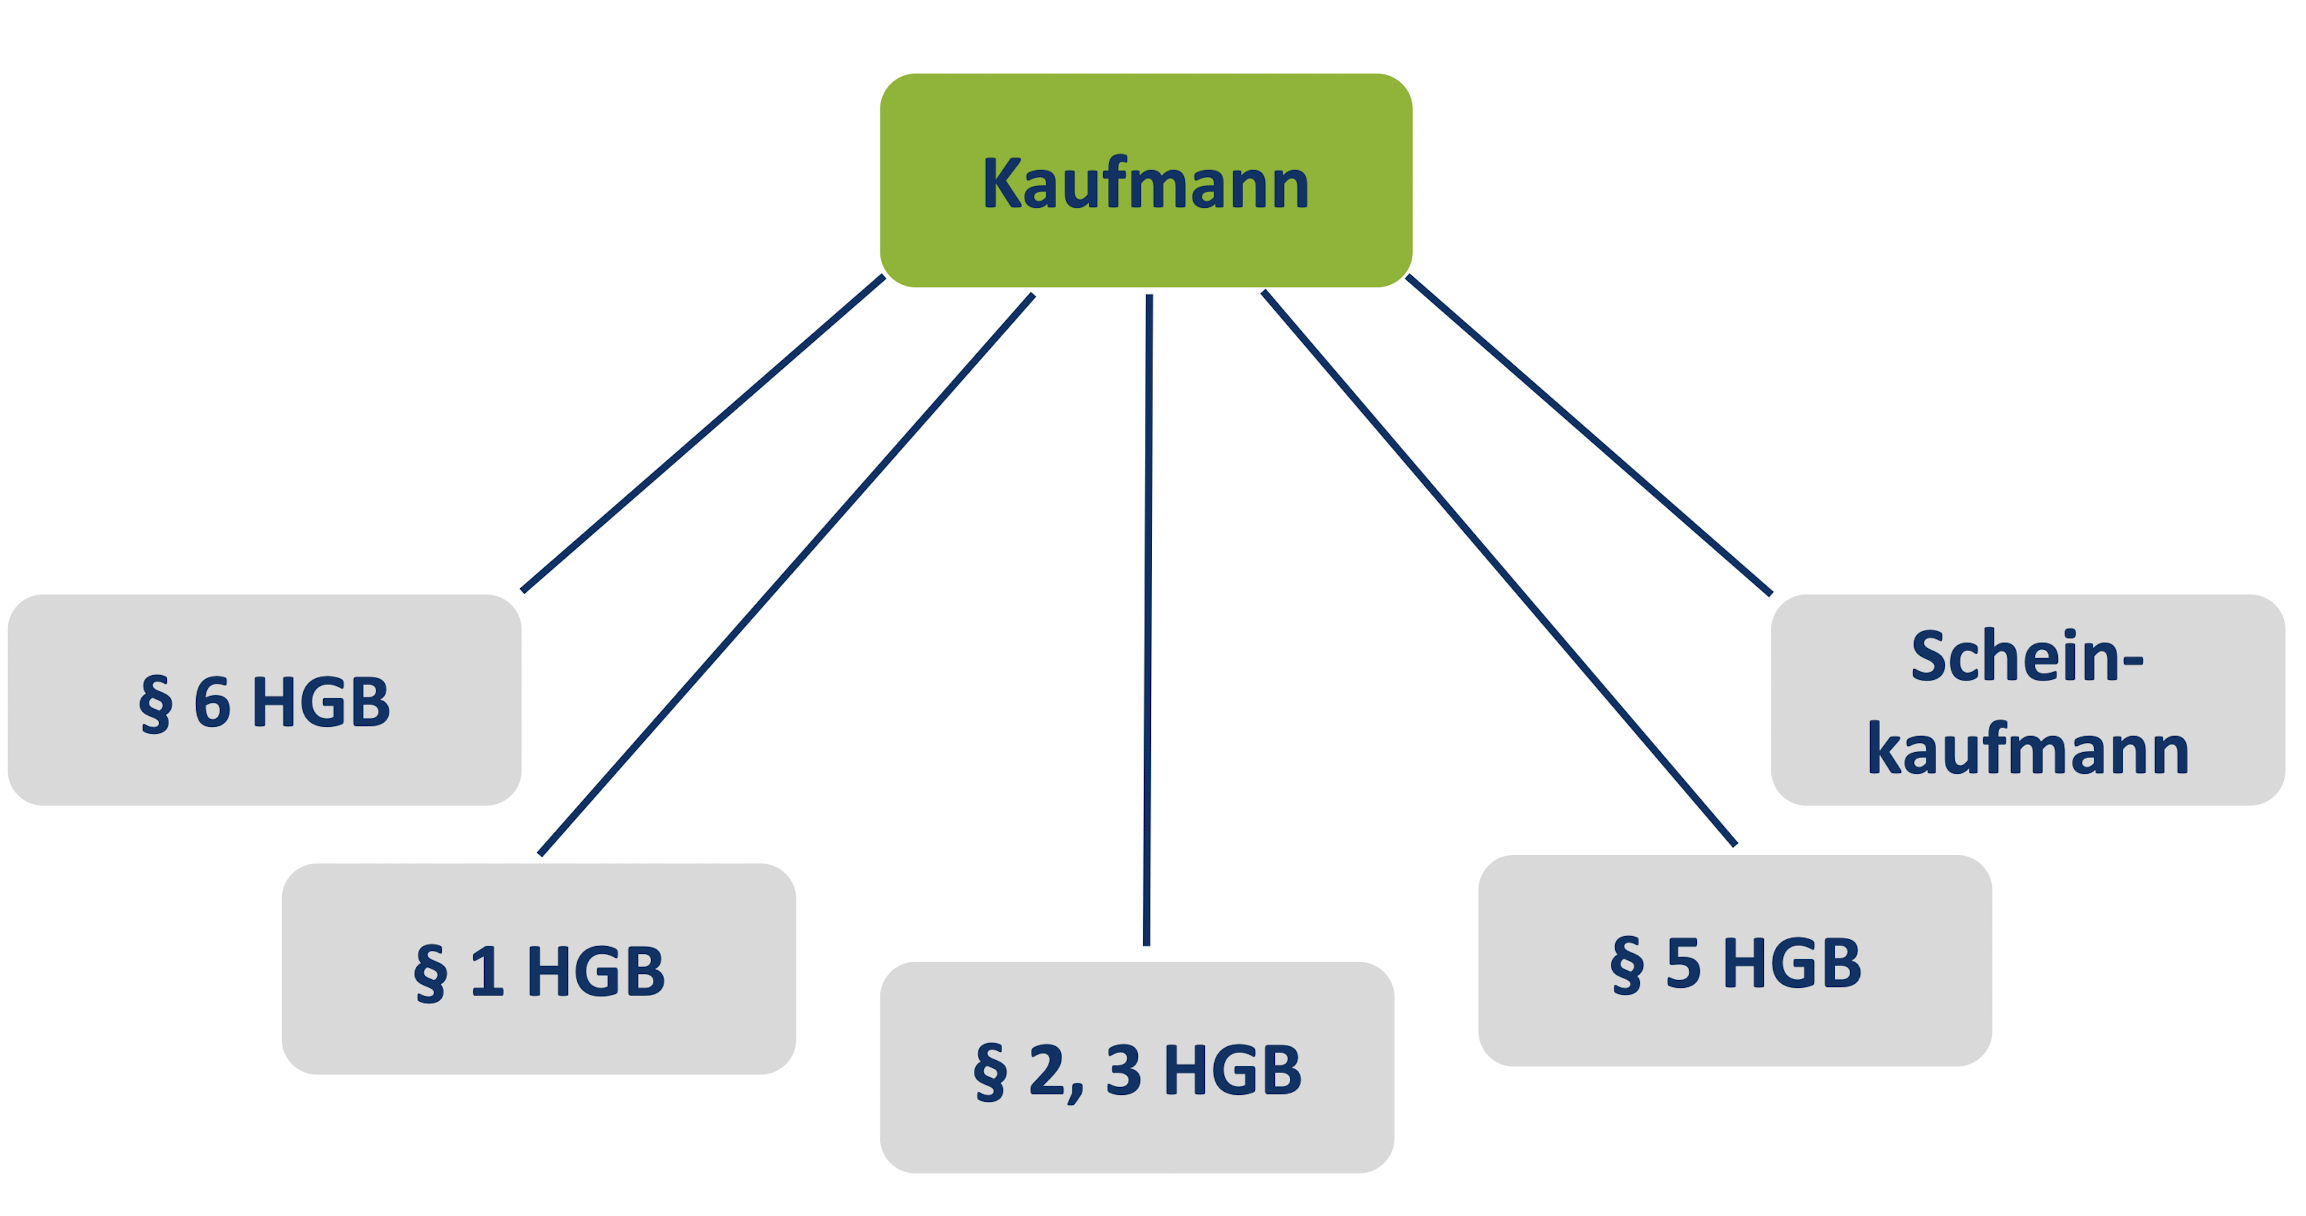
\includegraphics[width=0.5\linewidth]{Bildschirmfoto 2024-10-30 um 17.05.46.png}
    \caption{Prüfungsreihenfolge}
    \label{fig:enter-label}
\end{figure}
\end{document}
